\documentclass{article}

\usepackage{tikz}

% tikz packages
\usetikzlibrary{
  positioning,
  shapes.misc,
  calc,
  graphs,
  arrows.meta,
}

\tikzset{
  node distance= 5mm and 5mm,
  text height=1.5ex,
  text depth=.25ex,
  shape=coordinate,
  >={Stealth[round]},
  every new ->/.style={
    shorten >=1pt,
    thick, 
    black!50, 
    text=black
  },
  graphs/every graph/.style={edges=rounded corners},
  node/.style={
    rectangle,
    minimum size=6mm,
    very thick,
  },
  nonterminal/.style={
    node,
    draw=red!50!black!50,
    top color=white,
    bottom color=red!50!black!20,
    font=\itshape,
  },
  terminal/.style={
    node,
    rounded corners=3mm,
    draw=black!50,
    top color=white,
    bottom color=black!20,
    font=\ttfamily,
  },
  hv path/.style={
    to path={-| (\tikztotarget)},
  },
  vh path/.style={
    to path={|- (\tikztotarget)},
  },
  skip loop/.style={
    to path={-- ++(0,#1) -| (\tikztotarget)},
  },
}

\begin{document}
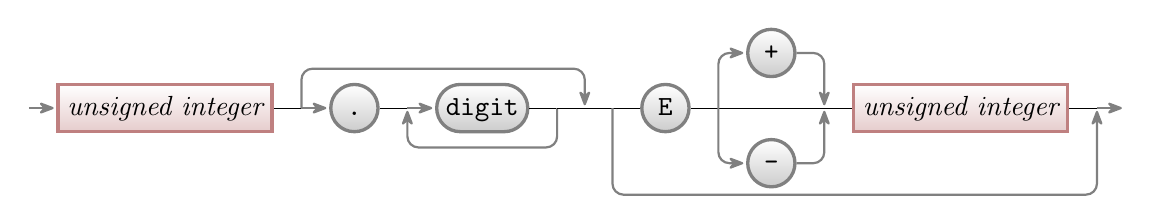
\begin{tikzpicture}
  \graph [grow right sep, branch down=7mm, simple] {
    / -> unsigned integer [nonterminal] -- p1 -> "." [terminal] -- p2 -> 
    digit [terminal] -- p3 -- p4 -- p5 -- E [terminal] -- q1 -> [vh path]
    { [nodes={yshift=7mm}]
      "+" [terminal], q2, "-" [terminal],
    } -> [hv path]
    q3                             --
    /unsigned integer[nonterminal] --
    p6                             ->
    /;

    p1 ->[skip loop=5mm] p4;
    p3 ->[skip loop=-5mm] p2;
    p5 ->[skip loop=-11mm] p6;

    q1 -- q2 -- q3;
  };
\end{tikzpicture}
\end{document}